
%% bare_conf.tex
%% V1.3
%% 2007/01/11
%% by Michael Shell
%% See:
%% http://www.michaelshell.org/
%% for current contact information.
%%
%% This is a skeleton file demonstrating the use of IEEEtran.cls
%% (requires IEEEtran.cls version 1.7 or later) with an IEEE conference paper.
%%
%% Support sites:
%% http://www.michaelshell.org/tex/ieeetran/
%% http://www.ctan.org/tex-archive/macros/latex/contrib/IEEEtran/
%% and
%% http://www.ieee.org/

%%*************************************************************************
%% Legal Notice:
%% This code is offered as-is without any warranty either expressed or
%% implied; without even the implied warranty of MERCHANTABILITY or
%% FITNESS FOR A PARTICULAR PURPOSE! 
%% User assumes all risk.
%% In no event shall IEEE or any contributor to this code be liable for
%% any damages or losses, including, but not limited to, incidental,
%% consequential, or any other damages, resulting from the use or misuse
%% of any information contained here.
%%
%% All comments are the opinions of their respective authors and are not
%% necessarily endorsed by the IEEE.
%%
%% This work is distributed under the LaTeX Project Public License (LPPL)
%% ( http://www.latex-project.org/ ) version 1.3, and may be freely used,
%% distributed and modified. A copy of the LPPL, version 1.3, is included
%% in the base LaTeX documentation of all distributions of LaTeX released
%% 2003/12/01 or later.
%% Retain all contribution notices and credits.
%% ** Modified files should be clearly indicated as such, including  **
%% ** renaming them and changing author support contact information. **
%%
%% File list of work: IEEEtran.cls, IEEEtran_HOWTO.pdf, bare_adv.tex,
%%                    bare_conf.tex, bare_jrnl.tex, bare_jrnl_compsoc.tex
%%*************************************************************************

% *** Authors should verify (and, if needed, correct) their LaTeX system  ***
% *** with the testflow diagnostic prior to trusting their LaTeX platform ***
% *** with production work. IEEE's font choices can trigger bugs that do  ***
% *** not appear when using other class files.                            ***
% The testflow support page is at:
% http://www.michaelshell.org/tex/testflow/



% Note that the a4paper option is mainly intended so that authors in
% countries using A4 can easily print to A4 and see how their papers will
% look in print - the typesetting of the document will not typically be
% affected with changes in paper size (but the bottom and side margins will).
% Use the testflow package mentioned above to verify correct handling of
% both paper sizes by the user's LaTeX system.
%
% Also note that the "draftcls" or "draftclsnofoot", not "draft", option
% should be used if it is desired that the figures are to be displayed in
% draft mode.
%
\documentclass[conference]{IEEEtran}
% Add the compsoc option for Computer Society conferences.
%
% If IEEEtran.cls has not been installed into the LaTeX system files,
% manually specify the path to it like:
% \documentclass[conference]{../sty/IEEEtran}


% Some very useful LaTeX packages include:
% (uncomment the ones you want to load)
\usepackage{graphicx}
\usepackage{amsmath, amssymb}
\usepackage[noadjust]{cite}
\usepackage{filecontents}
\usepackage[parfill]{parskip}

% *** MISC UTILITY PACKAGES ***
%
%\usepackage{ifpdf}
% Heiko Oberdiek's ifpdf.sty is very useful if you need conditional
% compilation based on whether the output is pdf or dvi.
% usage:
% \ifpdf
%   % pdf code
% \else
%   % dvi code
% \fi
% The latest version of ifpdf.sty can be obtained from:
% http://www.ctan.org/tex-archive/macros/latex/contrib/oberdiek/
% Also, note that IEEEtran.cls V1.7 and later provides a builtin
% \ifCLASSINFOpdf conditional that works the same way.
% When switching from latex to pdflatex and vice-versa, the compiler may
% have to be run twice to clear warning/error messages.






% *** CITATION PACKAGES ***
%
%\usepackage{cite}
% cite.sty was written by Donald Arseneau
% V1.6 and later of IEEEtran pre-defines the format of the cite.sty package
% \cite{} output to follow that of IEEE. Loading the cite package will
% result in citation numbers being automatically sorted and properly
% "compressed/ranged". e.g., [1], [9], [2], [7], [5], [6] without using
% cite.sty will become [1], [2], [5]--[7], [9] using cite.sty. cite.sty's
% \cite will automatically add leading space, if needed. Use cite.sty's
% noadjust option (cite.sty V3.8 and later) if you want to turn this off.
% cite.sty is already installed on most LaTeX systems. Be sure and use
% version 4.0 (2003-05-27) and later if using hyperref.sty. cite.sty does
% not currently provide for hyperlinked citations.
% The latest version can be obtained at:
% http://www.ctan.org/tex-archive/macros/latex/contrib/cite/
% The documentation is contained in the cite.sty file itself.






% *** GRAPHICS RELATED PACKAGES ***
%
\ifCLASSINFOpdf
  % \usepackage[pdftex]{graphicx}
  % declare the path(s) where your graphic files are
  % \graphicspath{{../pdf/}{../jpeg/}}
  % and their extensions so you won't have to specify these with
  % every instance of \includegraphics
  % \DeclareGraphicsExtensions{.pdf,.jpeg,.png}
\else
  % or other class option (dvipsone, dvipdf, if not using dvips). graphicx
  % will default to the driver specified in the system graphics.cfg if no
  % driver is specified.
  % \usepackage[dvips]{graphicx}
  % declare the path(s) where your graphic files are
  % \graphicspath{{../eps/}}
  % and their extensions so you won't have to specify these with
  % every instance of \includegraphics
  % \DeclareGraphicsExtensions{.eps}
\fi
% graphicx was written by David Carlisle and Sebastian Rahtz. It is
% required if you want graphics, photos, etc. graphicx.sty is already
% installed on most LaTeX systems. The latest version and documentation can
% be obtained at: 
% http://www.ctan.org/tex-archive/macros/latex/required/graphics/
% Another good source of documentation is "Using Imported Graphics in
% LaTeX2e" by Keith Reckdahl which can be found as epslatex.ps or
% epslatex.pdf at: http://www.ctan.org/tex-archive/info/
%
% latex, and pdflatex in dvi mode, support graphics in encapsulated
% postscript (.eps) format. pdflatex in pdf mode supports graphics
% in .pdf, .jpeg, .png and .mps (metapost) formats. Users should ensure
% that all non-photo figures use a vector format (.eps, .pdf, .mps) and
% not a bitmapped formats (.jpeg, .png). IEEE frowns on bitmapped formats
% which can result in "jaggedy"/blurry rendering of lines and letters as
% well as large increases in file sizes.
%
% You can find documentation about the pdfTeX application at:
% http://www.tug.org/applications/pdftex





% *** MATH PACKAGES ***
%
%\usepackage[cmex10]{amsmath}
% A popular package from the American Mathematical Society that provides
% many useful and powerful commands for dealing with mathematics. If using
% it, be sure to load this package with the cmex10 option to ensure that
% only type 1 fonts will utilized at all point sizes. Without this option,
% it is possible that some math symbols, particularly those within
% footnotes, will be rendered in bitmap form which will result in a
% document that can not be IEEE Xplore compliant!
%
% Also, note that the amsmath package sets \interdisplaylinepenalty to 10000
% thus preventing page breaks from occurring within multiline equations. Use:
%\interdisplaylinepenalty=2500
% after loading amsmath to restore such page breaks as IEEEtran.cls normally
% does. amsmath.sty is already installed on most LaTeX systems. The latest
% version and documentation can be obtained at:
% http://www.ctan.org/tex-archive/macros/latex/required/amslatex/math/





% *** SPECIALIZED LIST PACKAGES ***
%
%\usepackage{algorithmic}
% algorithmic.sty was written by Peter Williams and Rogerio Brito.
% This package provides an algorithmic environment fo describing algorithms.
% You can use the algorithmic environment in-text or within a figure
% environment to provide for a floating algorithm. Do NOT use the algorithm
% floating environment provided by algorithm.sty (by the same authors) or
% algorithm2e.sty (by Christophe Fiorio) as IEEE does not use dedicated
% algorithm float types and packages that provide these will not provide
% correct IEEE style captions. The latest version and documentation of
% algorithmic.sty can be obtained at:
% http://www.ctan.org/tex-archive/macros/latex/contrib/algorithms/
% There is also a support site at:
% http://algorithms.berlios.de/index.html
% Also of interest may be the (relatively newer and more customizable)
% algorithmicx.sty package by Szasz Janos:
% http://www.ctan.org/tex-archive/macros/latex/contrib/algorithmicx/




% *** ALIGNMENT PACKAGES ***
%
%\usepackage{array}
% Frank Mittelbach's and David Carlisle's array.sty patches and improves
% the standard LaTeX2e array and tabular environments to provide better
% appearance and additional user controls. As the default LaTeX2e table
% generation code is lacking to the point of almost being broken with
% respect to the quality of the end results, all users are strongly
% advised to use an enhanced (at the very least that provided by array.sty)
% set of table tools. array.sty is already installed on most systems. The
% latest version and documentation can be obtained at:
% http://www.ctan.org/tex-archive/macros/latex/required/tools/


%\usepackage{mdwmath}
%\usepackage{mdwtab}
% Also highly recommended is Mark Wooding's extremely powerful MDW tools,
% especially mdwmath.sty and mdwtab.sty which are used to format equations
% and tables, respectively. The MDWtools set is already installed on most
% LaTeX systems. The lastest version and documentation is available at:
% http://www.ctan.org/tex-archive/macros/latex/contrib/mdwtools/


% IEEEtran contains the IEEEeqnarray family of commands that can be used to
% generate multiline equations as well as matrices, tables, etc., of high
% quality.


%\usepackage{eqparbox}
% Also of notable interest is Scott Pakin's eqparbox package for creating
% (automatically sized) equal width boxes - aka "natural width parboxes".
% Available at:
% http://www.ctan.org/tex-archive/macros/latex/contrib/eqparbox/





% *** SUBFIGURE PACKAGES ***
%\usepackage[tight,footnotesize]{subfigure}
% subfigure.sty was written by Steven Douglas Cochran. This package makes it
% easy to put subfigures in your figures. e.g., "Figure 1a and 1b". For IEEE
% work, it is a good idea to load it with the tight package option to reduce
% the amount of white space around the subfigures. subfigure.sty is already
% installed on most LaTeX systems. The latest version and documentation can
% be obtained at:
% http://www.ctan.org/tex-archive/obsolete/macros/latex/contrib/subfigure/
% subfigure.sty has been superceeded by subfig.sty.



%\usepackage[caption=false]{caption}
%\usepackage[font=footnotesize]{subfig}
% subfig.sty, also written by Steven Douglas Cochran, is the modern
% replacement for subfigure.sty. However, subfig.sty requires and
% automatically loads Axel Sommerfeldt's caption.sty which will override
% IEEEtran.cls handling of captions and this will result in nonIEEE style
% figure/table captions. To prevent this problem, be sure and preload
% caption.sty with its "caption=false" package option. This is will preserve
% IEEEtran.cls handing of captions. Version 1.3 (2005/06/28) and later 
% (recommended due to many improvements over 1.2) of subfig.sty supports
% the caption=false option directly:
%\usepackage[caption=false,font=footnotesize]{subfig}
%
% The latest version and documentation can be obtained at:
% http://www.ctan.org/tex-archive/macros/latex/contrib/subfig/
% The latest version and documentation of caption.sty can be obtained at:
% http://www.ctan.org/tex-archive/macros/latex/contrib/caption/




% *** FLOAT PACKAGES ***
%
%\usepackage{fixltx2e}
% fixltx2e, the successor to the earlier fix2col.sty, was written by
% Frank Mittelbach and David Carlisle. This package corrects a few problems
% in the LaTeX2e kernel, the most notable of which is that in current
% LaTeX2e releases, the ordering of single and double column floats is not
% guaranteed to be preserved. Thus, an unpatched LaTeX2e can allow a
% single column figure to be placed prior to an earlier double column
% figure. The latest version and documentation can be found at:
% http://www.ctan.org/tex-archive/macros/latex/base/



%\usepackage{stfloats}
% stfloats.sty was written by Sigitas Tolusis. This package gives LaTeX2e
% the ability to do double column floats at the bottom of the page as well
% as the top. (e.g., "\begin{figure*}[!b]" is not normally possible in
% LaTeX2e). It also provides a command:
%\fnbelowfloat
% to enable the placement of footnotes below bottom floats (the standard
% LaTeX2e kernel puts them above bottom floats). This is an invasive package
% which rewrites many portions of the LaTeX2e float routines. It may not work
% with other packages that modify the LaTeX2e float routines. The latest
% version and documentation can be obtained at:
% http://www.ctan.org/tex-archive/macros/latex/contrib/sttools/
% Documentation is contained in the stfloats.sty comments as well as in the
% presfull.pdf file. Do not use the stfloats baselinefloat ability as IEEE
% does not allow \baselineskip to stretch. Authors submitting work to the
% IEEE should note that IEEE rarely uses double column equations and
% that authors should try to avoid such use. Do not be tempted to use the
% cuted.sty or midfloat.sty packages (also by Sigitas Tolusis) as IEEE does
% not format its papers in such ways.

% *** PDF, URL AND HYPERLINK PACKAGES ***
%
%\usepackage{url}
% url.sty was written by Donald Arseneau. It provides better support for
% handling and breaking URLs. url.sty is already installed on most LaTeX
% systems. The latest version can be obtained at:
% http://www.ctan.org/tex-archive/macros/latex/contrib/misc/
% Read the url.sty source comments for usage information. Basically,
% \url{my_url_here}.

% *** Do not adjust lengths that control margins, column widths, etc. ***
% *** Do not use packages that alter fonts (such as pslatex).         ***
% There should be no need to do such things with IEEEtran.cls V1.6 and later.
% (Unless specifically asked to do so by the journal or conference you plan
% to submit to, of course. )

% correct bad hyphenation here
\hyphenation{op-tical net-works semi-conduc-tor}

\begin{document}
%
% paper title
% can use linebreaks \\ within to get better formatting as desired
\title{Energy Forecasting for the Global Energy Forecasting Competition 2014\\[10pt]\Large{\emph{Semester Project Report}}}

% author names and affiliations
% use a multiple column layout for up to three different
% affiliations
\author{\IEEEauthorblockN{Fabian Brix\\MSc Candidate}
\IEEEauthorblockA{School of Computer \& Communication Sciences\\
Swiss Federal Institute of Technology Lausanne\\
fabian.brix@epfl.ch}
%\and
%\IEEEauthorblockN{Homer Simpson}
%\IEEEauthorblockA{Twentieth Century Fox\\
%Springfield, USA\\
%Email: homer@thesimpsons.com}
}

% conference papers do not typically use \thanks and this command
% is locked out in conference mode. If really needed, such as for
% the acknowledgment of grants, issue a \IEEEoverridecommandlockouts
% after \documentclass

% for over three affiliations, or if they all won't fit within the width
% of the page, use this alternative format:
% 
%\author{\IEEEauthorblockN{Michael Shell\IEEEauthorrefmark{1},
%Homer Simpson\IEEEauthorrefmark{2},
%James Kirk\IEEEauthorrefmark{3}, 
%Montgomery Scott\IEEEauthorrefmark{3} and
%Eldon Tyrell\IEEEauthorrefmark{4}}
%\IEEEauthorblockA{\IEEEauthorrefmark{1}School of Electrical and Computer Engineering\\
%Georgia Institute of Technology,
%Atlanta, Georgia 30332--0250\\ Email: see http://www.michaelshell.org/contact.html}
%\IEEEauthorblockA{\IEEEauthorrefmark{2}Twentieth Century Fox, Springfield, USA\\
%Email: homer@thesimpsons.com}
%\IEEEauthorblockA{\IEEEauthorrefmark{3}Starfleet Academy, San Francisco, California 96678-2391\\
%Telephone: (800) 555--1212, Fax: (888) 555--1212}
%\IEEEauthorblockA{\IEEEauthorrefmark{4}Tyrell Inc., 123 Replicant Street, Los Angeles, California 90210--4321}}

% use for special paper notices
%\IEEEspecialpapernotice{(Invited Paper)}

% make the title area
\maketitle

\begin{abstract}
%\boldmath
The abstract goes here.
\end{abstract}
% IEEEtran.cls defaults to using nonbold math in the Abstract.
% This preserves the distinction between vectors and scalars. However,
% if the conference you are submitting to favors bold math in the abstract,
% then you can use LaTeX's standard command \boldmath at the very start
% of the abstract to achieve this. Many IEEE journals/conferences frown on
% math in the abstract anyway.

% no keywords

% For peer review papers, you can put extra information on the cover
% page as needed:
% \ifCLASSOPTIONpeerreview
% \begin{center} \bfseries EDICS Category: 3-BBND \end{center}
% \fi
%
% For peerreview papers, this IEEEtran command inserts a page break and
% creates the second title. It will be ignored for other modes.
\IEEEpeerreviewmaketitle

\section{Introduction}
\subsection{GEFCom 2014}
The Global Energy Forecasting Competition (GEFCom 2014) is the second edition of a competition first held on Kaggle in 2012 that attracted hundreds of participants contributing many novel ideas to the energy forecasting field. The second edition lasted from 08/15/2014 to 12/15/2014 and was sponsored by several IEEE bodies and the International Journal of Forecasting. It included four competition tracks: electric load, electricity price, wind power and solar power forecasting. The respective data was published on the community platform of crowdanalytix.com on a weekly basis during the competition. The format of the competition was that of rolling forecasting requiring contestants to submit the next period of interest to forecast a day before the next set of data was published. To appear on the final leaderboard the contestants had to submit 99 quantiles for each step throughout the forecast horizon. In the course of this semester project we focused solely on the electric load forecasting track. This track had a weekly forecast horizon of one month and consisted of three trial periods and twelve competitive periods. In order to feature on the final leaderboard nine competitive submissions were required. Due to our lack of familiarity with the subject, participating in the competition was not prioritized after initial attempts. Instead the focus was on comparison of the performance of different methods on the whole dataset via cross validation.
%The topic of the probabilistic electric load forecasting track is to forecast the probabilistic distribution (in quantiles) of the hourly loads for one utility on a rolling basis
%Historical Data Release (Competition Starts) 8/15/2014
%Evaluation Period Starts 9/14/2014
%Registration Deadline 10/10/2014
%Evaluation Period Ends 12/6/2014
%Final Report and Code Due (Competition Ends) 12/15/2015

\subsection{Short Introduction to Energy Load Forecasting}
Before we review related work we are going to introduce the area of Energy Load Forecasting. Load forecasting, as it is commonly referred to, is usually concerned with the prediction of hourly, daily, weekly, and annual values of the system demand and peak demand of an electric utility \cite{Fan2010}. Such forecasts are sometimes categorized as short-term (up to 1 week), medium-term (1 week - 1 year) and long-term (> 1 year ) forecasts, depending on the time horizon. In the load forecasting track of GEFCom 2014 we are concerned with forecasting the daily electricity demand/load of a utility for a whole month on a rolling basis given the data of the previous years. The task is therefore on the threshold between short-term and medium-term load forecasting.\par
Load Forecasting is necessary for the planning of energy system and their effective operation and maintenance. Forecasting accuracy therefore has a major impact on electric utilities and their regulators. In case of overestimation of future load/energy demand utility providers will operate too many units possibly driving energy demand and in case of long-term forecasts investment in the construction of new infrastructure can be wasted. Underestimation leads ot unmet demand and systems that are vulnerable to crashes.  
The output of such forecasts can either be point forecasts or estimates of the probability distribution of values of future demand as required during GEFCom 2014.
Electricity demands follow a nonlinear, volatile pattern subject to several exogenous variables such weather conditions, randomness in human behavior leading to randomness in demand and economic conditions and demographic changes. In GEFCom 2014 the exogenous variables are limited to weather conditions in the form of recorded temperature at several sites and calendar effects such as the effects of weekends and holidays on the electricity demand.
In this report we analyse the predictions produced by algorithms that are capable of capturing the nonlinear dependencies between these exogeneous variables and the load such as General Additive Models, Random Forests, Multilayer Perceptrons. We do not strive to build any algorithms ourselves, but employ the various implementations in R of the mentioned algorithms.

\section{Review of Related Work}
Review previous work from Gefcom 2012 and beyond including papers with related approaches including but not necessarily limited to those that can be found under the following link: http://blog.drhongtao.com/2014/08/recommended-papers-for-gefcom2014-contestants.html. Distinguish between approaches to temperature and load prediction.\par
Probabilistic Electric Load Forecasting: A Tutorial Review
%https://onedrive.live.com/view.aspx?resid=BCA4C2DC57A4CB2A!519&app=WordPdf
contains literature review for longterm probabilistic load forecasting

Tao Hang, Jason Wilson:
Long Term Probabilistic Load Forecasting and Normalization With Hourly Information
but papers is on Long Term Electric Load Forecasting: 1-X years \cite{Hong2014Normalization}

Rob Hyndman, Shu Fan
Density Forecasting for Longterm Electricity Demand
Source for calendar effects \cite{Hyndman2010}

Shu Fan, Rob Hyndman
Short-term load forecasting based on a semi-parametric additive model \cite{Fan2010}

\section{Dataset and Evaluation Metrics}
\subsection{Dataset}
%Forecast horizon: 1 month
The dataset provided by GEFCom 2014 includes hourly historical load and weather data of a utility in an undisclosed area on the east coast of the United States of America. The 25 weather stations in the dataset provide historical temperature for their respective zones. However, the load data consists only of the system level load in Mega Watts (MW) and not all of the zonal level load series. Therefore, forecasts in the context of Smart Grid Technology are not required. The temperature data made available consists of 25 series of temperature data in Fahrenheit from the 25 different weather statios dating from 01/01/2001 to 12/01/2011. The load data of the utility is recorded starting from the 01/01/2005 at 1am.\par
The complete data set acted both as training and validation set except for the first and last month of the data published for the reason that the data was released on a weekly basis. It consists of 15 spreadhseets in the format of Comma-Seperated Values (CSV) for the load forecasting track. The first spreadsheet contains data starting from 01/01/2001 up until midnight on the 10/01/2014 at 1am from when on the incremental spreadsheets released every week contain only one month of data.\par
The forecasts were required to be made starting from 10/01/2010 on a monthly rolling basis for 15 months. The nature of the data provided required the contestants to produce their own temperature forecasts for the month ahead in the dataset.\par

\subsection{Evaluation Metrics}
The Evaluation Metric employed to score the contestants' submissions of quantile forecasts is the tilted loss/error function also known as the pinball loss/error function. In the following paragraphs let $y$ denote an observation and $\hat{y}$ denote a corresponding forecast while $\xi$ is defined as the residual $y-\hat{y}$.\par
TODO: Include short explanation.
\[
  L_{\tau}(\xi)=\begin{cases} \tau \xi & \text{if } \xi \geq 0 \\
                                          (\tau-1)\xi & \text{if } \xi < 0 
                                  \end{cases} \quad\text{where } \xi=(y-\hat{y})
\]
%\tau ist Steigung wenn \xi>=0 und Gefälle wenn \xi<0

\begin{figure}[ht!]
\centering
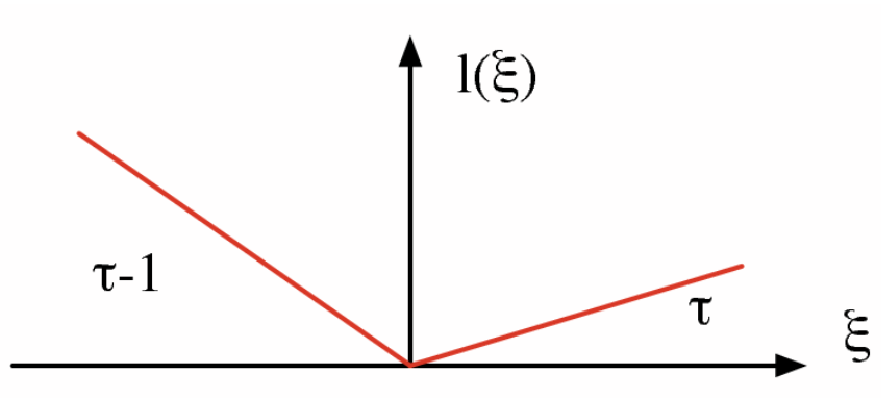
\includegraphics[width=\linewidth]{gfx/pinball.pdf}
\caption{The tilted loss function for 50th, $\tau=0.5$, and 75th, $\tau=0.75$, quantile \cite{Takeuchi2005}.}
\label{fig:pinball}
\end{figure}
TODO: Include the proof for why the ``pinball'' loss estimates the $\tau$-quantile \cite{Takeuchi2005}.\par
In our evaluation of forecasts, we further use some well-established point error metrics, for the simple reason that we generate our quantile predictions starting from a point prediction. The measures are the Mean Average Error (MAE), Root Mean Squared Error (RMSE) and Mean Absolute Percentage Error (MAPE).\par
The MAE and RMSE measures are the two most common scale-dependent errors, meaning that the residuals $\xi_i$ (for ith observations) are on the same scale as the data. Hence, MAE and RMSE are in units of Fahrenheit or Mega Watt for our data set. 
\[
  \text{MAE}=\mathbb{E}[\xi_i]
\]
\[
  \text{RMSE}=\sqrt{\mathbb{E}[\xi_i]}
\]
As a percentage error the MAPE measure is scale-independent. In our case it is useful for giving an immediate sense of the relative magnitude? of the error.
\[
  \text{MAPE}=\mathbb{E}\left[\left| \frac{100\xi_i}{y_i} \right|\right]
\]
The measure is undefined for $y_i=0$. Fortunately, in our dataset all values are several integers larger than zero for both load and temperature series so that the measure is neither undefined or affected by extreme values.
%source: Rob Hyndman, Forecasting principles and practice, https://www.otexts.org/fpp/2/5

\subsection{Data Cleaning}
An annoying feature of the dataset is that the timestamps are not saved in the international ISO 8601 standard, but as ``MMddYYYY H:m'' without leading zeros for both days and months. Fortunately, the dataset was provided continuously without gaps and therefore the problem could be easily solved by hard-coding the first and last datetimes and using these to generate the needed sequence of datetimes.n
%found a way to automatically solve the problem through the linkedin group and a question a participant asked on stackoverflow (http://stackoverflow.com/questions/25386730/parsing-ambiguous-timestamps). 
%However, had to make slight modifications to make it work
%Still didn't work 100%, lost one week on this

\subsection{Data Selection}
%$Corr_X(m) = \frac{\mathbb{E}\[X_t-\mu_x)(X_{t+m})\]}{\var_X}$
The Cross Correlations of the temperature series of the 25 weather stations suggest that they can be explained to over 90\% by the first series.\par
[include correlation plots here]\par
A temperature of 60 degrees Fahrenheit would therefore allow for an error of maximum 6 degrees of Fahrenheit or 3 degrees Celsius respectively. As we will see later in this report this error is negligable when taking into account the inaccuracy of/the error introduced in the temperature prediction.


\section{Feature Selection}
Description of features obtained from the data. 
Name all features in this part or only the ones in the final selection? 

Use this part to motivate selection of time of year (TOY) variable:\par
The effect of the lag on the Time Series Correlation Coefficient can be demonstrated using the Autocorrelation function acf() of the R stats package. Here we display five plots showing the Autocorrelation Function for different maximum lags: 
\begin{figure}[h!]
\centering
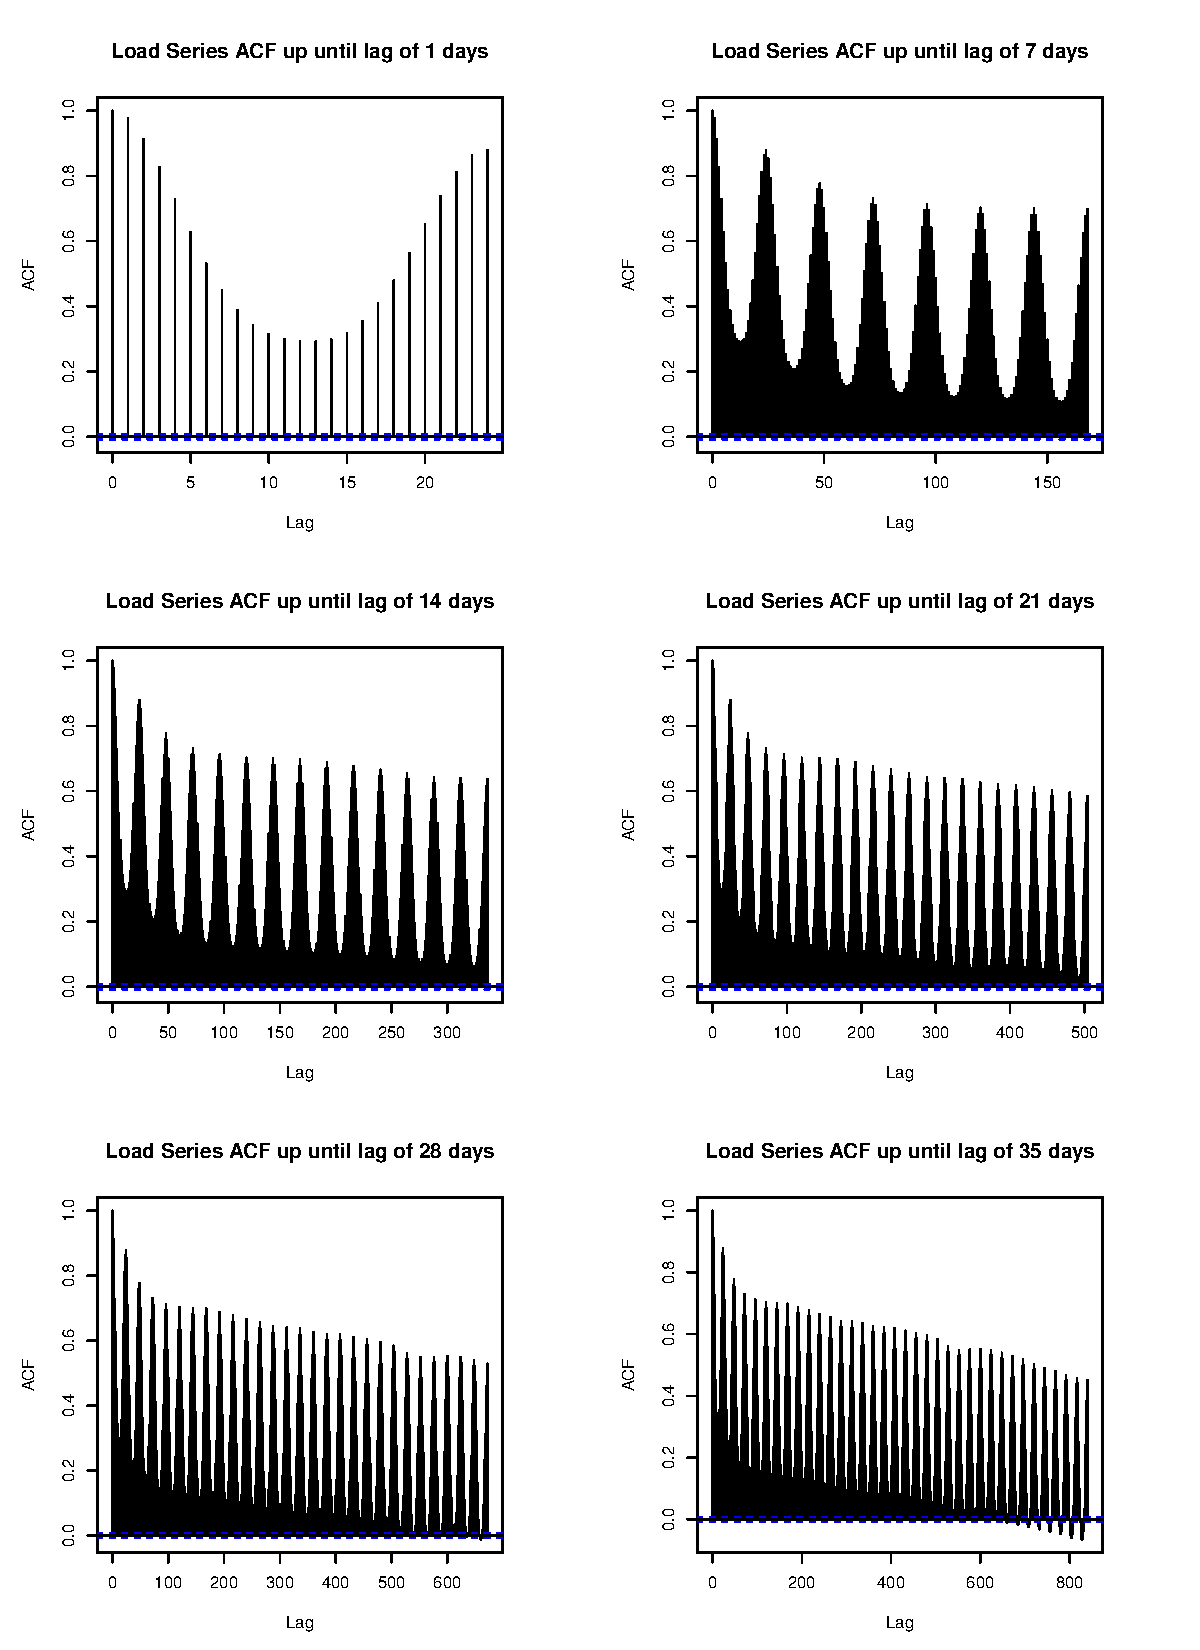
\includegraphics[width=\linewidth]{../data/analysis/acf-load-lag-var-days_font.pdf}
\caption{Plots of Autocorrelation Function Estimates for hourly load data in MW for different maximum lags.}
\label{fig:load-acf}
\end{figure}
As can be seen the correlation diminishes exponentially up until a lag of 72h from any point in the time series, then stays more or less constant for up to 7-8 days, whereafter it diminishes near linearly (up to a lag of 35 days).\par 
Autocorrelation plots for temperature and load side by side for one year (daily avg)\par
include seasonal decompositions?

\subsection{Calendar Features}
hour, TOY vs. month
\cite{Fan2010}
\cite{Hyndman2010}

\section{Models}
Description of the Models (LM), GAM (more extensive), NN, RF

\section{Analysis}
What combination of features and models for temperature and load provide us with a good prediction accuracy with respect to Gefcom leaderboard?

\subsection{Temperature Modeling}
\subsubsection{Data Processing}
average temperature vs. principal component

\subsubsection{Effect on Load Prediction}
Effect of temperature on load prediction evaluated using different methods:\\
Mean over past years (yearly lag), LM, GAM, NN, RF vs. true temperature

\subsubsection{Evaluate Results of weekly vs. monthly Temperature Prediction}
plot MAPE \& PINBALL scores for different methods over load training + CV period in a 1x2 plot of the form:\\
monthly scores \quad weekly scores

\subsection{Load Modeling}

\subsubsection{Evaluate the Influence of the Lag on Load Prediction}
set the basis by plotting MAPE \& PINBALL scores by week over w1, w2, w3, w4; one curve for every month in CV\\
do this for every method\\
as well as a comparison of the best performing configuration of every method among each other\\

\subsubsection{Evaluate Performance for different Method Configurations}
Use temp method that provides best score as shown in Temperature Modeling Section\par
Different GAM formulas:\\
plot MAPE \& PINBALL scores for all GAM formulas over CV period in a 2x2 plot of the form:\\
monthly load with monthly temp \quad monthly load with weekly temp\\
weekly load with monhtly temp \quad weekly load with weekly temp\par
\vspace*{5pt}
Different NN hidden units:\\
plot MAPE \& PINBALL scores in 2x2 plot\par
Different RF ntrees:\\ 
plot MAPE \& PINBALL scores in 2x2 plot\par

\subsubsection{Compare Performance of different Methods}
choose best scoring configuration for every method and plot the results in one 2x2 plot

% An example of a floating figure using the graphicx package.
% Note that \label must occur AFTER (or within) \caption.
% For figures, \caption should occur after the \includegraphics.
% Note that IEEEtran v1.7 and later has special internal code that
% is designed to preserve the operation of \label within \caption
% even when the captionsoff option is in effect. However, because
% of issues like this, it may be the safest practice to put all your
% \label just after \caption rather than within \caption{}.
%
% Reminder: the "draftcls" or "draftclsnofoot", not "draft", class
% option should be used if it is desired that the figures are to be
% displayed while in draft mode.
%
%\begin{figure}[!t]
%\centering
%\includegraphics[width=2.5in]{myfigure}
% where an .eps filename suffix will be assumed under latex, 
% and a .pdf suffix will be assumed for pdflatex; or what has been declared
% via \DeclareGraphicsExtensions.
%\caption{Simulation Results}
%\label{fig_sim}
%\end{figure}

% Note that IEEE typically puts floats only at the top, even when this
% results in a large percentage of a column being occupied by floats.


% An example of a double column floating figure using two subfigures.
% (The subfig.sty package must be loaded for this to work.)
% The subfigure \label commands are set within each subfloat command, the
% \label for the overall figure must come after \caption.
% \hfil must be used as a separator to get equal spacing.
% The subfigure.sty package works much the same way, except \subfigure is
% used instead of \subfloat.
%
%\begin{figure*}[!t]
%\centerline{\subfloat[Case I]\includegraphics[width=2.5in]{subfigcase1}%
%\label{fig_first_case}}
%\hfil
%\subfloat[Case II]{\includegraphics[width=2.5in]{subfigcase2}%
%\label{fig_second_case}}}
%\caption{Simulation results}
%\label{fig_sim}
%\end{figure*}
%
% Note that often IEEE papers with subfigures do not employ subfigure
% captions (using the optional argument to \subfloat), but instead will
% reference/describe all of them (a), (b), etc., within the main caption.


% An example of a floating table. Note that, for IEEE style tables, the 
% \caption command should come BEFORE the table. Table text will default to
% \footnotesize as IEEE normally uses this smaller font for tables.
% The \label must come after \caption as always.
%
%\begin{table}[!t]
%% increase table row spacing, adjust to taste
%\renewcommand{\arraystretch}{1.3}
% if using array.sty, it might be a good idea to tweak the value of
% \extrarowheight as needed to properly center the text within the cells
%\caption{An Example of a Table}
%\label{table_example}
%\centering
%% Some packages, such as MDW tools, offer better commands for making tables
%% than the plain LaTeX2e tabular which is used here.
%\begin{tabular}{|c||c|}
%\hline
%One & Two\\
%\hline
%Three & Four\\
%\hline
%\end{tabular}
%\end{table}


% Note that IEEE does not put floats in the very first column - or typically
% anywhere on the first page for that matter. Also, in-text middle ("here")
% positioning is not used. Most IEEE journals/conferences use top floats
% exclusively. Note that, LaTeX2e, unlike IEEE journals/conferences, places
% footnotes above bottom floats. This can be corrected via the \fnbelowfloat
% command of the stfloats package.



\section{Conclusion}
The conclusion goes here.




% conference papers do not normally have an appendix


% use section* for acknowledgement
\section*{Acknowledgment}




% trigger a \newpage just before the given reference
% number - used to balance the columns on the last page
% adjust value as needed - may need to be readjusted if
% the document is modified later
%\IEEEtriggeratref{8}
% The "triggered" command can be changed if desired:
%\IEEEtriggercmd{\enlargethispage{-5in}}

% references section

% can use a bibliography generated by BibTeX as a .bbl file
% BibTeX documentation can be easily obtained at:
% http://www.ctan.org/tex-archive/biblio/bibtex/contrib/doc/
% The IEEEtran BibTeX style support page is at:
% http://www.michaelshell.org/tex/ieeetran/bibtex/
%\bibliographystyle{IEEEtran}
% argument is your BibTeX string definitions and bibliography database(s)
%\bibliography{IEEEabrv,../bib/paper}
%
% <OR> manually copy in the resultant .bbl file
% set second argument of \begin to the number of references
% (used to reserve space for the reference number labels box)
\bibliographystyle{IEEEtran}
\bibliography{references}{}

% \begin{thebibliography}{1}

% \bibitem{IEEEhowto:kopka}
% H.~Kopka and P.~W. Daly, \emph{A Guide to \LaTeX}, 3rd~ed.\hskip 1em plus
%   0.5em minus 0.4em\relax Harlow, England: Addison-Wesley, 1999.

% \end{thebibliography}

\end{document}


